%% Note I have taken the template form %%
%% Chris Carmona: carmona@stats.ox.ac.uk %%

\documentclass{beamer}

%load any additional packages

\usepackage[UKenglish]{babel}
\usepackage[utf8]{inputenc} % so we can input characters with accents (e.g. ő)

\usepackage{st}

\usepackage{graphicx} % ease graphics management
\graphicspath{{images/}} % define folder with images
\usefonttheme{serif} % change font to allow \textbf{}
\usepackage{charter} % Nicer fonts

\usepackage{amsmath,amsthm,amssymb} % for math equations

\usepackage{natbib} % richer citation
\usepackage{breakcites} % avoid overfull hbox for long cites


\usepackage{bbm}
\usepackage{amssymb}
\usepackage{bbm}
\usepackage{amsmath}

\usepackage{mathrsfs}
\newcommand\norm[1]{\left\lVert#1\right\rVert}
\newcommand*\by{{\times}}

% \addtobeamertemplate{navigation symbols}{}{%
%     \usebeamerfont{footline}%
%     \usebeamercolor[fg]{footline}%
%     \hspace{1em}%
%     \insertframenumber/\inserttotalframenumber
% }

% \setbeamertemplate{footline}[text line]{%
%   \parbox{0.8\linewidth}{
%     \vspace*{-8pt}\insertshorttitle~(\insertshortauthor)
%   }
%   \hfill%
%   \parbox{0.15\linewidth}{
%     \vspace*{-8pt}\raggedleft\insertpagenumber
%   }
% }

\setbeamertemplate{footline}[text line]{%
  \parbox{\linewidth}{\vspace*{-8pt} TUM
  \hfill\insertshorttitle
  \hfill\insertpagenumber}}
\setbeamertemplate{navigation symbols}{}


%% Information (author, title, etc.) %%

\title[Johnson-Lindenstrauss Lemma and Restricted Isometry Property]{% short title for footer
    Johnson-Lindenstrauss Lemma and Restricted Isometry Property
    \vspace{0.5cm}
}

\author{ Grigor Keropyan}
% \supervisor{ Vazgen Mikayelyan}

\institute{
        \textit{Department of Mathematics}\\
        \textit{Mathematics in Data Science} \\
        \textit{Technische Universität München (TUM)}
        \vspace{0.5cm}
}
\date[Venue and Date]{% short date for footer
    July, 2021
}


%% Content of slides %%
%%%%%%%%%%%%%%%%%%%% 
\begin{document}
%%%%%%%%%%%%%%%%%%%%

% Title slide %
{
    \setbeamertemplate{footline}{}
    \setbeamertemplate{headline}{}
    \setbeamercolor{background canvas}{bg=oxfordblue}
    \maketitle
}

%----------------------------%
% Contents slide
\begin{frame}
\frametitle{Outline}
\tableofcontents
\end{frame}
%----------------------------%

%now include the slides
\setbeamercovered{transparent}
%----------------------------%
\section{Introduction}

\section{Johnson-Lindenstrauss (JL) Lemma}

\begin{frame}{Johnson-Lindenstrauss Lemma 1}
    \begin{figure}
        \centering
        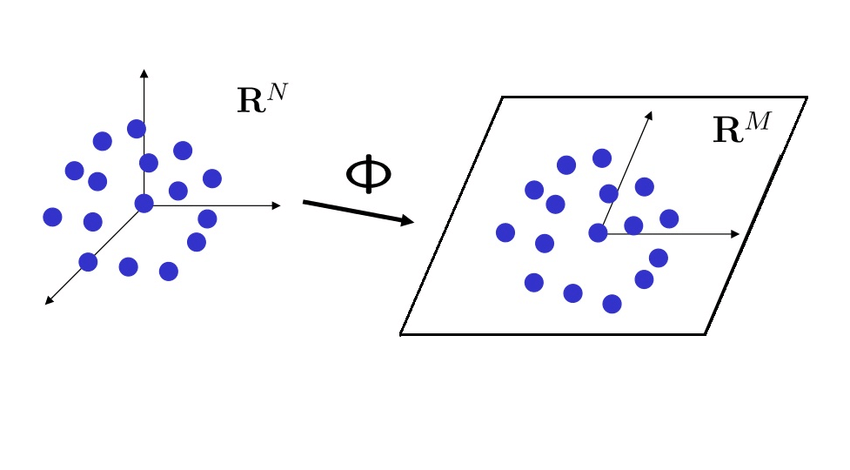
\includegraphics[width=9cm]{images/jl_mapping1.png}
        \caption{Mapping from high dimensional space on lower dimensional space}
        \label{fig:jl_mapping1}
    \end{figure}
\end{frame}

\begin{frame}{Johnson-Lindenstrauss Lemma 2}

    \begin{figure}
        \centering
        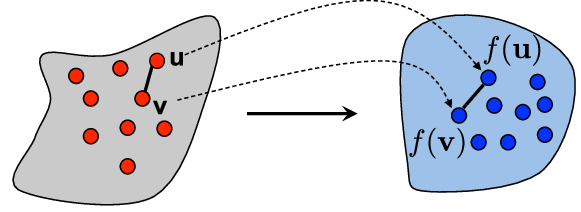
\includegraphics[width=9cm]{images/jl_mapping2.png}
        \caption{Mapping from high dimensional space on lower dimension by keeping relative distances}
        \label{fig:jl_mapping2}
    \end{figure}
    
\end{frame}

\begin{frame}{Johnson-Lindenstrauss Lemma 3}

\noindent
{\bf Lemma 4} (Johnson-Lindenstrauss) (Lemma 4.1 in \citep{isometry}) \\
{\it
Let $\epsilon \in (0, 1)$ is given and $N \in \mathbb{N}$. For every set $\mathcal{Q} \in \mathbb{R}^N$, if $n$ is a positive integer such that $n \ge n_0 := O(ln(\#\mathcal{Q})/\epsilon^2)$, there exists a Lipschtz mapping $f : \mathbb{R}^N \rightarrow \mathbb{R}^n$ such that 
\begin{equation}
\label{eqn:jl}
(1 - \epsilon) \norm{u - v}_2^2 \leq \norm{f(u) - f(v)}_2^2 \leq (1 + \epsilon) \norm{u - v}_2^2,
\end{equation}
for all $u, v \in \mathcal{Q}$.
}
    
\end{frame}

\section{Concentration Inequality}

\begin{frame}{Concentration Inequality}

    {\bf Definition 2} \\
{\it Let $\Phi \in \mathbb{R}^{n \by N}$ be a random matrix and for any $x \in \mathbb{R}^N$ expectation of random variable $\norm{\Phi(x)}_2^2$ is $\norm{x}_2^2$, that is 
$$
\mathbb{E}[\norm{\Phi(x)}_2^2] = \norm{x}_2^2,
$$
where $n, N \in \mathbb{N}$. We say that random matrix $\Phi$ satisfies concentration inequality if the random variable $\norm{\Phi(x)}_2^2$ is strongly concentrated about its expected value, that is
$$
\mathbb{P}(|\norm{\Phi(x)}_2^2 - \norm{x}_2^2| \geq \epsilon\norm{x}_2^2) \leq 2e^{-nc(\epsilon)}, \quad 0 \le \epsilon \le 1, 
$$
where $\epsilon$ is a constant and $c(\epsilon)$ is also a constant depends only on $\epsilon$ such that for all $\epsilon \in (0, 1)$, $c(\epsilon) \ge 0$.
} \\
\end{frame}

\begin{frame}{Concentration Inequality: Examples 1}

Entries $\Phi_{i, j}$ of $\Phi$ are independent samples from Normal distribution $$
    \{\Phi_{i, j}\}_{i \in [n], j \in [N]} \stackrel{i.i.d}{\sim} \mathcal{N}(0, \frac{1}{n}).
    $$
    
\end{frame}

\begin{frame}{Concentration Inequality: Examples 2}
Entries $\Phi_{i, j}$ of $\Phi$ are independent samples from following distribution 
    $$
    X :=\begin{cases}
         +1/\sqrt{n} & \text{with probability } 1/2, \\
         -1/\sqrt{n} & \text{with probability } 1/2.
    \end{cases}
    $$
    
\end{frame}

\begin{frame}{Concentration Inequality: Examples 3}
Entries $\Phi_{i, j}$ of $\Phi$ are independent samples from following distribution 
    $$
    X :=\begin{cases}
         +\sqrt{3}/\sqrt{n} & \text{with probability } 1/6, \\
         0 & \text{with probability } 2/3, \\
         -\sqrt{3}/\sqrt{n} & \text{with probability } 1/6.
    \end{cases}
    $$
    
    In all the above examples the constant $c(\epsilon)$ can be chosen as $\epsilon^2/4 - \epsilon^3/6$. \\
    
\end{frame}


\section{Restricted Isometry Property (RIP)}

\begin{frame}{Restricted Isometry Property 1}
    \begin{figure}
        \centering
        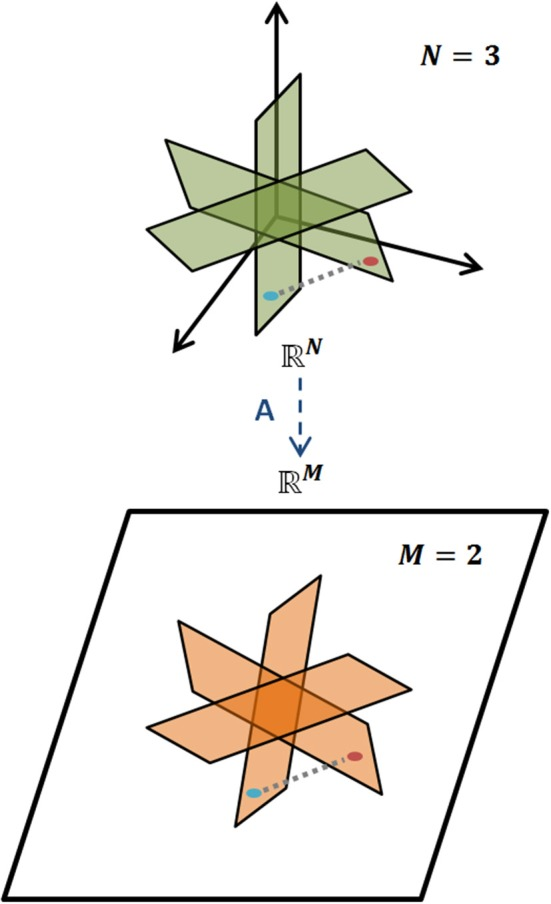
\includegraphics[width=9cm, height=7cm]{images/rip1.png}
        \caption{RIP mapping}
        \label{fig:rip1}
    \end{figure}
\end{frame}

\begin{frame}{Restricted Isometry Property 2}
\noindent
{\bf Definition 3} \\
{\it
We say that a matrix $\Phi$ satisfies Restricted Isometry Property (RIP) of order $k$ and level $\delta \in (0, 1)$ (concisely, $(k, \delta)-RIP$) if 
\begin{equation}
\label{eqn:rip}
    (1-\delta) \norm{x}_2^2 \leq \norm{\Phi(x)}_2^2 \leq (1+\delta) \norm{x}_2^2 \quad \forall k-\text{sparse } x \in \mathbb{R}^N.
\end{equation}
The restricted isometry constant $\delta_k$ is defined as the smallest value of $\delta$ for which (\ref{eqn:rip}) holds.
}
    
\end{frame}


\section{Connection between JL Lemma and RIP}

\begin{frame}{JL Lemma implies RIP}
\noindent
{\bf Theorem 4} (Theorem 5.2 in \citep{isometry}) \\
{\it
Let $n, N \in \mathbb{N}, \delta \in (0, 1)$ and $\Phi \in \mathbb{R}^{n \by N}$ be a random matrix which satisfies concentration inequality (see Definition 2), then $\exists c_1, c_2 > 0$ depending only on $\delta$ such that $\Phi$ satisfies Restricted Isometry Property of order $k \leq c_1n/log(N/k)$ and level $\delta$ with probability $ \geq 1 - 2e^{-c_2n}$.
}
\end{frame}

\begin{frame}{Proof idea of Theorem 4}
\begin{enumerate}
    \item For each index set $T$ with $\#T = k$ there is finite set of points $\mathcal{Q}_T \subseteq X_T$ such that $\norm{q}_2 = 1,$ $\forall q \in \mathcal{Q}_T$ and $\forall x \in X_T$ with $\norm{x}_2 = 1$ we have 
\begin{equation}
\label{eqn:iso_cover}
    min_{q \in \mathcal{Q}_T} \norm{x-q}_2 \leq \delta/4.
\end{equation}
such that $\# \mathcal{Q}_T \leq (12/\delta)^k$.
\pause
    \item Using 1. prove 
    \begin{equation}
\label{eqn:iso1}    
(1 - \delta) \norm{x}_2 \leq \norm{\Phi(x)}_2 \leq (1 + \delta) \norm{x}_2, \quad \forall x \in X_T,
\end{equation}
with high probability.
\pause
    \item Using union bound with 2. prove RIP
    \begin{equation}
(1 - \delta) \norm{x}_2 \leq \norm{\Phi(x)}_2 \leq (1 + \delta) \norm{x}_2 \quad \forall k-\text{sparse } x \in \mathbb{R}^N,
    \end{equation}
with high probability. 
\end{enumerate}
    
\end{frame}

\begin{frame}{RIP implies JL Lemma (1)}
\begin{enumerate}
    \item Matrices that satisfy RIP are not random!
    
    \item How can we randomize a matrix?
\end{enumerate}

\end{frame}

\begin{frame}{RIP implies JL Lemma (2)}
    \noindent
{\bf Definition 5} \\
{\it We call $\xi \in \mathbb{R}^N$ as a Rademacher sequence if it is uniformly distributed on $\{-1, +1\}^N$, where $N \in \mathbb{N}$. } 
\\[1cm] \pause
For a matrix $\Phi$ we might consider random matrix $\Phi D_{\xi}$, where $\xi$ is a Rademacher sequence and $D_{\xi}$ is a diagonal matrix with entries from $\xi$

\end{frame} 


\begin{frame}{RIP implies JL Lemma (3)}

\noindent
{\bf Theorem 6} (Theorem 3.1 in \citep{Khramer}) \\
{\it
Let $\eta > 0, \epsilon \in (0, 1), n, N \in \mathbb{N}$ be given and the set $E \subset \mathbb{R}^N$ has cardinality $p := \#E$. Suppose the matrix $\Phi \in \mathbb{R}^{n \by N}$ satisfies Restricted Isometry Property of order $k \geq 40log\frac{4p}{\eta}$ and level $\delta \leq \frac{\epsilon}{4}$. Taking $\xi \in \mathbb{R}^N$ as a Rademacher sequence we have 
\begin{equation}
    \label{eqn:iso_jl1}
    (1 - \epsilon) \norm{x}_2^2 \leq \norm{\Phi D_{\xi}x}_2^2 \leq (1 + \epsilon) \norm{x}_2^2,
\end{equation}
for all $x \in E$, with probability
$$
 \geq 1- \eta.
$$
}
    
\end{frame}

\begin{frame}{Proof idea of Theorem 6 (1)}
    \begin{enumerate}[1]
        \item Split matrices by column wise blocks
        \begin{equation}
    \label{eqn:iso_jl4}
    \begin{split}
    \norm{\Phi D_{\xi}x}_2^2 & = \norm{\Phi D_{x}\xi}_2^2 \\
    & = \sum_{J=1}^R \norm{\Phi_{(J)} D_{(x_{(J)})} \xi_{(J)}}_2^2 \\
    & + 2 \xi_{(1)}^* D_{x_{(1)}} \Phi_{(1)}^* \Phi_{(-1)} D_{x_{(-1)}} \xi_{(-1)} \\
    & + \sum_{J,L = 2, J \not = L }^R \langle \Phi_{(J)} D_{x_{(J)}} \xi_{(J)}, \Phi_{(L)} D_{x_{(L)}} \xi_{(L)} \rangle.
    \end{split}
\end{equation}
    \end{enumerate}
\end{frame}

\begin{frame}{Proof idea of Theorem 6 (2)}
    \begin{enumerate}[2] 
        \item Get bounds for every item in the right hand side of equation (\ref{eqn:iso_jl4})
        \pause
        \begin{enumerate}
            \item  Deterministic bound on the first item
            \begin{equation}
    \label{eqn:iso_jl5}
    (1 - \epsilon/4) \norm{x}_2^2 \leq \sum_{J=1}^R \norm{\Phi_{(J)} D_{x_{(J)}} \xi_{(J)}}_2^2 \leq (1 + \epsilon/4) \norm{x}_2^2.
    \end{equation} \pause
     \item Probabilistic bound on the second item
        \begin{equation}
        \label{eqn:iso_jl7}
        \mathbb{P}(\exists x \in E: |2 \xi_{(1)}^* D_{x_{(1)}} \Phi_{(1)}^* \Phi_{(-1)} D_{x_{(-1)}} \xi_{(-1)}| \geq 0.2 \epsilon) \leq \frac{\eta}{2}
        \end{equation} \pause
         \item Probabilistic bound on the third item
       \begin{equation}
        \label{eqn:iso_jl8}
        \mathbb{P}(\exists x \in E: |\sum_{J,L = 2, J \not = L }^R \langle \Phi_{(J)} D_{x_{(J)}} \xi_{(J)}, \Phi_{(L)} D_{x_{(L)}} \xi_{(L)} \rangle| \geq 0.55 \epsilon) \leq \eta/2
        \end{equation}
        \end{enumerate} 
      
    \end{enumerate}
\end{frame}

\begin{frame}{Proof idea of Theorem 6 (2)}
\begin{enumerate} [3]
    \item Putting everything together
    \begin{equation}
        \mathbb{P}(\exists x \in E: |\norm{\Phi D_{\xi}x}_2^2/\norm{x}_2^2 - 1| \geq  \epsilon) \leq \eta.
    \end{equation}
\end{enumerate}
    
\end{frame}


\begin{frame}
\centering
    Thank you!
\end{frame}

% References slide
\begin{frame}
\frametitle{references}
\small
\bibliographystyle{apalike} %use the apalike bibliography style
\bibliography{references} % bibliography file
\end{frame}

%%%%%%%%%%%%%%%%%%%%
\end{document}
%%%%%%%%%%%%%%%%%%%%
